
\chapter{Getting started}
\label{txt:gettingstarted}

Once you have your Tellervo desktop application installed (see chapter \ref{txt:installation}) and you also have access to a Tellervo server (either via your lab network administrator or your own on as a Virtual Appliance) you are ready to start using Tellervo.  Below are some basic instructions for performing common tasks in Tellervo followed by a number of more in-depth chapters.  If you are running Tellervo with database integration disabled (Tellervo-lite mode) then see section \ref{txt:tellervolite} for further details.

\section{Measuring a new sample}
\index{Sample!Measuring|(}
\label{txt:new}
Once your measuring platform has been configured, measuring your first sample is simple.  To start a new measurement go to \menutwo{File}{New} or click the `new' icon on the home screen. A dialog will appear where you can scan your sample's barcode, or press the button to enter metadata for your sample later. Barcodes minimize data entry errors and also speed up the process of measuring your samples. See section \ref{txt:barcodes} for more information. Once you have scanned your barcode or pressed the button, you will then be presented with an empty Tellervo metadata screen.

The next step is to fill out the metadata information. If you have used a barcode, nearly all of this metadata will be filled in for you, otherwise you will need to fill this out yourself. Details about metadata can be found in chapter \ref{txt:metadata}, page \pageref{txt:metadata}.  Once you have populated the metadata tab, you can then switch to the data tab (figure \ref{fig:datascreen}).  

\begin{figure}[hbtp]
  \centering
    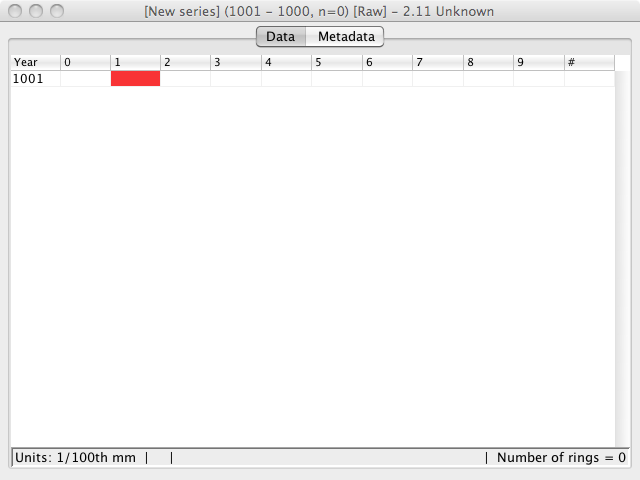
\includegraphics[width=0.6\textwidth]{Images/datascreen.png}
    \caption{An empty data window ready to receive measurements.  Note the status bar at the bottom includes buttons for changing the measurement variable, display units and cumulative statistics.  The data table stores ring width values in decadal rows following the standard convention which derives from data entry via punch-cards.  Undated sequences begin in the relative year 1001 for the same reason.}
    \label{fig:datascreen}
\end{figure}

Before you begin measuring you need to tell Tellervo what sort of measurements you are making: whole ring widths; or early/latewood widths (the default is whole ring widths).  To specify early/latewood widths you need to go to \menuthree{Edit}{Measuring mode\ldots}{Early and latewood widths}.  If you use this menu after you have already measured some rings you will be warned that Tellervo will delete the data you have already collected.  Once in `early and latewood widths' measuring mode you will be able to choose which data is displayed in the table by clicking the variable box on the status line and choose between: Ring width; Earlywood width; Latewood width; Early/Latewood width.

To begin measuring your sample you can now go to \menutwo{Edit}{Start measuring}, press the start measuring button on the toolbar, or you can press F5. While measuring you should be provided with audible feedback for each ring measured with a more pronounced sound made every 10th ring. If there is a problem communicating with your measuring hardware, check your settings in the preferences dialog. If you still have problems contact the Tellervo developers by going to \menutwo{Help}{Report bug on last transaction}, making sure you include your email address and any further information.

If your sample is already dated and/or you already know how many rings your sample has, then you can initialise your data matrix using the button on the toolbar.  This gives you a dialog requesting date and ring number information which can be useful for those of you that use the skeleton plotting method prior to measuring.  

Note by default Tellervo labels rings as relative years beginning in 1001.  If your sample is dated, you should explicity tell Tellervo either using the initialise grid function prior to measuring, or by going to \menutwo{Tools}{Redate} once you've finished.

Depending on the measuring platform hardware you have, you will see some variation of the measuring panel in figure \ref{fig:measurepanel}. The left display holds the absolute position of the last ring boundary (for device that measure cumulatively), the middle display holds the last recorded measurement width and the right display holds the current position of the measuring plaform (for devices that report live measurements).  The right-hand display is useful for devices that don't have a physical display such as the Lintab. 

\begin{wrapfigure}{r}{0.5\textwidth}
  \begin{center}
    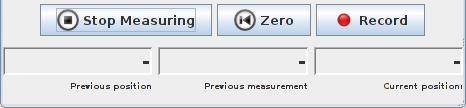
\includegraphics[width=70mm]{Images/measurepanel.png}
  \end{center}
  \caption{Measuring control panel.}
  \label{fig:measurepanel}
\end{wrapfigure}


Tellervo supports the measuring of rings both individually and cumulatively.  We feel that it is easier and more accurate to measure rings individually, that is to say the device is reset to zero after each measurement.  If a device accepts requests to reset measurements (e.g.\ Quadra Chek boxes) or if it automatically resets itself to zero after recording a measurement (e.g.\ EVE IO) then this procedure is used by Tellervo.  In this case the user begins measuring by setting the display to zero, then turns the platform to the end of the ring, then either presses the `measure' button on the hardware device or the `record' button on the screen.

\tip{If your device does not have a physical `measure' button you don't need to click on the `record' button each time.  Instead click on the `turn on mouse trigger' button and then you can use your mouse's left button as a measure button regardless of where the mouse is on the screen. This means you don't need to lift your eyes from your microscope to ensure you are clicking the button correctly.  When you're finished measuring press escape to exit this mode.}

Certain devices (e.g. Boekler Microcode boxes) do not listen for requests to reset to zero.  In this case to measure each ring individually, you would need to manually reset the reading to zero following each measurement.  This would of course be extremely tedious.  In this situation Tellervo measures cumulatively from the beginning of the first ring and calculates the ring width based on the previous ring boundary position.  With this method you must be careful not to knock your sample, and you must also take special care when altering radii to navigate around problem structures.  If you do knock your sample, the best way to recover is to reset your platform to zero and press the measure button.  Next, press the `stop measuring button', manually fix the values in the data table, then begin measuring again from where you left off.

If you are in `Early and latewood widths' measuring mode the measurements are made and sent to the data table in pairs.  The first measurement should be of the earlywood of the ring, and the next value the latewood measurement.  Whether you are currently measuring early or latewood is indicated as a message at the bottom of the measuring panel.

\index{Ring remarks}
While you measure your sample you can flag features in a ring by right clicking on any cell in the table and selecting one or more of the standard notes (see figure \ref{fig:ringremarks}).

Tellervo supports all standard TRiDaS remarks including: fire damage; frost damage; crack; false ring(s); compression wood; tension wood; traumatic ducts; single pinned; double pinned; triple pinned and many others.  Rings that include remarks are indicated by the relevant icon in the data screen.  Depending on your method of work, this can be useful for keeping track of sample pin holes.  For instance, if a missing or false ring is discovered after a sample has been pinholed, the offset in pinholes can be easily seen without resurfacing the sample.  

\begin{wrapfigure}{r}{0.5\textwidth}
  \begin{center}
    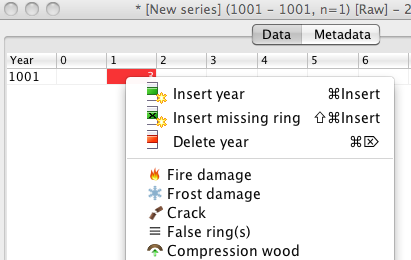
\includegraphics[width=0.42\textwidth]{Images/ringremarks.png}
  \end{center}
  \caption{Right click context menu showing some of the options for adding remarks to rings.}
  \label{fig:ringremarks}
\end{wrapfigure}

In addition to the right click menu, you can also access ring remarks by opening the remarks panel using the button on the toolbar.  This panel gives the the ability to add free text remarks to individual rings.  One final method for adding remarks is specific to fire history researchers.  Standard FHX-style remarks can be added to rings by pressing the equivalent FHX character code key in the relevant ring cells.  For instance pressing a lower-case `a' in a cell will add the `fire injury in latewood' remark.   

The data screen also contains a status bar at the bottom. By clicking on the units section, you can switch between micron and 1/100th mm units. Tellervo understands the units being supplied by the measuring platform, therefore changes here are purely for display purposes only. If you have a platform that measures in microns, but prefer to see the values in 1/100th mm then you can use this feature.  There are also options on the status bar that enable you to choose one of a variety of summary statistics about your series.

Once you have finished measuring your sample, you should then go to \menutwo{File}{Save} to save your series to the database. 
\index{Sample!Measuring|)}


\section{Opening existing data}
\index{Sample!Opening}
\label{txt:open}
If you have used traditional dendrochronology software, you are probably used to opening existing dendro data files from your computer.  Tellervo works in a different way.  All data accessed by Tellervo is stored within the central Tellervo database rather than in files.  The database provides many benefits over file based storage, most importantly it means there is a high degree of security and integrity in your data.\footnote{This doesn't mean you don't have to backup your data though!  Whoever is in charge of maintaining your Tellervo database should make sure regular backups are made--preferably offsite.}

To use data that you have stored in existing data files you must first \emph{import} your data into the Tellervo database.  This gives you the opportunity to clean-up your data!  For details of how to import your data see chapter \ref{txt:importExport}, page \pageref{txt:importExport}.

Once you have data in your database, either by importing existing data files or measuring new samples, you can access your data through the database browser.  This is accessed through the \menutwo{File}{Open} or \menutwo{File}{Open multiple} menus and an example of the dialog is shown in figure \ref{fig:dbbrowser}. The same database browser dialog is used in multiple places throughout Tellervo, e.g.\ when adding addition series to graphs and when choosing chronologies to crossdate against. 

\begin{figure}[hbtp]
  \centering
    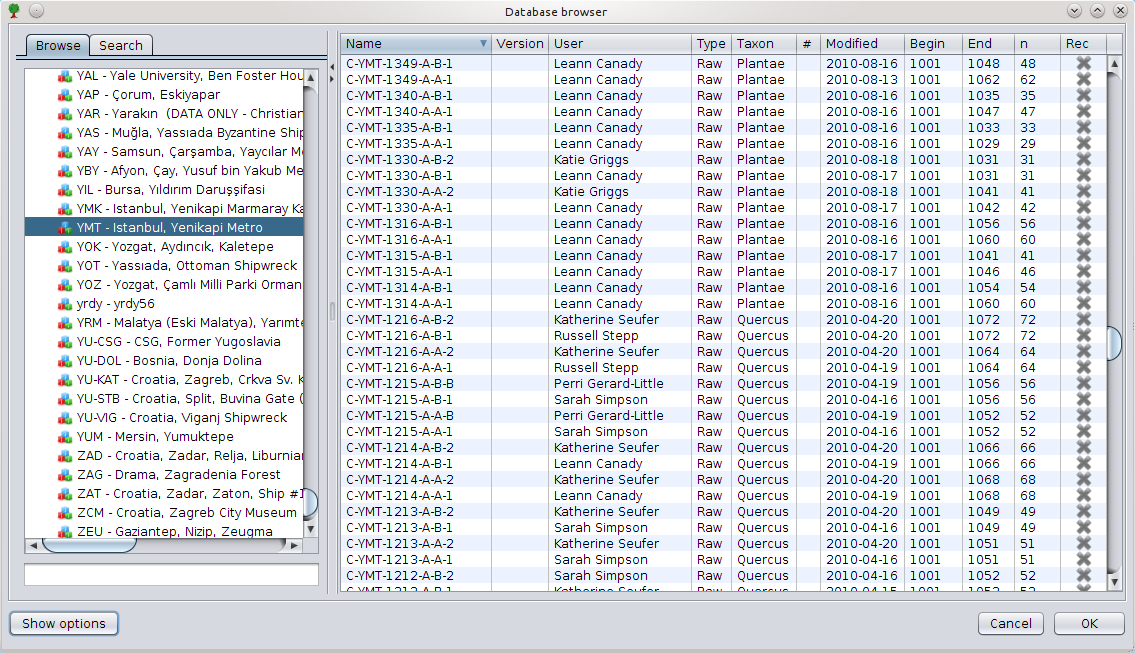
\includegraphics[width=0.9\textwidth]{Images/dbbrowser.png}
    \caption{Screenshot of the database browser dialog.}
    \label{fig:dbbrowser}
\end{figure}

The database browser is divided into two main parts.  On the left is the browse and search tabs, and on the right is the series table.  Selecting options in the browse or search tab populates the series table on the right with all the series that match the specified criteria.  

\warn{The search tab is currently a `work-in-progress' so we recommend you use the browse tab until further notice.}

The browse tab shows a heirarchical tree view of the contents of your Tellervo database based upon the TRiDaS data model.  The panel will be pre-populated with all the objects in your database but it is possible to `drill-down' by right clicking on an object and choosing `Expand branch'.  Expanding an object for instance, will show all the elements associated with that object, and expanding an element will show all the samples associated with the specified element.  To better understand the TRiDaS terminology please read chapter \ref{txt:metadata}, page \pageref{txt:metadata}.

By double clicking (or right clicking and choosing `Search for associated series') on an item in the browse panel Tellervo will search the database for all series that are associated with the specified entity.  The results of the search will be shown in the series table on the right of the screen.  This table shows basic metadata about each search and is sortable by click on any of the column headers.  To open a series, simply select one of these series and click `OK'.  If the database browser is open in 'multiple series' mode, then you can use the arrow buttons to select multiple series to open in one go.

There is also a `Show options' button on the database browser dialog.  This adds additional advanced methods for filtering the series table to help you find the data you are interested in.

\section{Reconciling data}
\index{Sample!Reconciling}
Tellervo has been developed not only for experience dendrochronologists, but as a tool for teaching students.  It therefore includes a comprehensive `reconciling' tool for supervisors to check the quality of measurements made by students.  The reconcile dialog does a comparison of a measurement series made by a student with a references series of the same radius measured by the supervisor.  The same dialog can also prove useful for comparing measurements from two experienced dendrochronologists when handling particularly difficult samples.


\section[Tellervo-lite]{Tellervo-lite: running without database server integration}
\label{txt:tellervolite}
\index{Tellervo-lite}
\index{Offline mode}
When you run Tellervo with database integration disabled (referred to as Tellervo-lite), you are presented with a simplified interface without database functionality. Tellervo-lite has basic measuring functionality only and does not take advantage of many of the advanced features introduced by the full Tellervo application.  We strongly recommend installing Tellervo server to take advantage of all that Tellervo has to offer.

When reading this manual please keep in mind that for the most part it is assuming that you are using the full Tellervo application.  Although in some cases the information is useful regardless of whether you're using Tellervo or Tellervo-lite, there will be differences, and of course features that require the database (such as mapping, user permissions and analysis tools) that will be disabled or missing entirely.  

Instead of opening and saving data to the Tellervo database, in Tellervo-lite data is accessed via traditional data file formats such as Tucson, Heidelberg and Sheffield etc.  In Tellervo-lite, \menutwo{File}{Open} presents the user with a standard file dialog box rather than the Tellervo database browser.  Similarly when the user clicks \menutwo{File}{New}, instead of being presented by the barcode dialog, they are taken directly to the data editor (with a limited metadata tab).   

Tellervo-lite is a departure from the primary mission of Tellervo (i.e.\ to provide a user-friendly application that supports standardised dendro data and metadata). The support for metadata in legacy dendro file formats ranges from non-existent to minimal with little standardisation.  Given the wide variation in metadata that can potentially be provided by these formats, it is not practical to support reading and editing in Tellervo-lite, instead it provides a very minimal interface for recording non-standardised metadata.  This basic metadata screen replaces the TRiDaS-based metadata interface normally seen in the standard version of Tellervo.  How this basic metadata is used (or indeed whether it is used at all) depends on the file format you choose to save to.  

When opening legacy dendro files in Tellervo-lite, it is possible that metadata will be discarded.  So if you open and edit an existing file in Tellervo, then overwrite the orignal you may well loose information.  We highly recommend saving changes to a different file.  It is also important for users to understand the limitations of the file formats you're reading from and writing to.  For instance the Tucson format has no mechanism for indicating whether years are absolute or relative so data loaded from Tucson files will be marked as relative years in Tellervo.  Some formats also store ring-width measurements in 1/100th mm integers, so if you measure in microns then the values will be rounded. A full description of each format along with their limitations is given in appendix \ref{txt:fileFormatsStart}.







